\documentclass{article}%
\usepackage[T2A]{fontenc}%
\usepackage[utf8]{inputenc}%
\usepackage{lmodern}%
\usepackage{textcomp}%
\usepackage{lastpage}%
\usepackage[russian]{babel}%
\usepackage{titling}%
\usepackage{nopageno}%
\usepackage{amsfonts}%
\usepackage{amssymb}%
\usepackage{amsmath}%
\usepackage[left=2cm,right=2cm, top=2cm,bottom=2cm]{geometry}%
\usepackage{circuitikz}%

\begin{document}%

\begin{titlepage}
  \begin{center}
    \large
    Министерство образования Республики Беларусь\\
    \vspace{0.5cm}
    БЕЛОРУССКИЙ ГОСУДАРСТВЕННЫЙ УНИВЕРСИТЕТ
    \vspace{0.5cm}
     
    Факультет прикладной математики и информатики
\bigskip
\vfill
\vfill
\vfill
\vfill
\centerline{\Large \bf Лабораторная работа 3}
    \vspace{0.5cm}
\centerline{"Численное решение смешанной задачи для уравнения теплопроводности"}
\end{center}

\vspace*{\fill}
\vfill
\vfill
\vfill
\hfill
\begin{minipage}{0.25\textwidth}
{   Подготовил:\\ студент 3 курса 3 группы\\ Тев Никита Михайлович\\}
\end{minipage}

\mbox{}
\vfill
\hfill
\begin{minipage}{0.25\textwidth}
  {\large{\bf Преподаватель: } 
{\it\\ Горбачёва Юлия \\ Николаевна}}
\end{minipage}

\vspace*{\fill}
\vfill
\vfill
\vfill
\vfill
\vfill
\vfill
\vfill
\vfill
\vfill
\vspace*{\fill}
\begin{center}
Минск, 2019 г.
\end{center}
\end{titlepage}

\begin{enumerate}%
\item%
\underline{Постановка задачи}

На сетке узлов $\overline{\omega}_{h\tau}$ найти численное решение смешанной задачи для одномерного уравнения теплопроводности с использованием:
\begin{itemize}
\item явной разностной схемы с $h=\tau=0.1$ и $h=0.1, \tau=\frac{h^2}{2}=0.005$;
\item чисто неявной разностной схемы с $h=\tau=0.1$;
\item разностной схемы Кранка-Николсона с $h=\tau=0.1$.
\end{itemize}
Выписать соответствующие разностные схемы, указать их порядок аппроксимации, указать, являются ли схемы абсолютно устойчивыми по начальным данным. 
Вычислить погрешность численного решения. 
Построить графики, демонстрирующие устойчивое и неустойчивое поведение явной разностной схемы.

\item%
\underline{Условие задачи:}

$\begin{cases} 
\frac{\partial u}{\partial t} = \frac{\partial^2 u}{\partial x^2} + cosx(cost+sint),\,  0<x<1,\, 0<t\le0.5 \\
u(x,0)=u_0(x)=0,\, 0\le x\le1 \\
u(0, t)=u_1(t)=sint,\, 0\le t\le0.5 \\
u(1, t)=u_2(t)=sin(t)cos(1),\, 0\le t\le0.5 \\
\end{cases}$

Точное решение: $u(x, t) = sin(t)cos(x)$

\item%
\underline{Сетка}

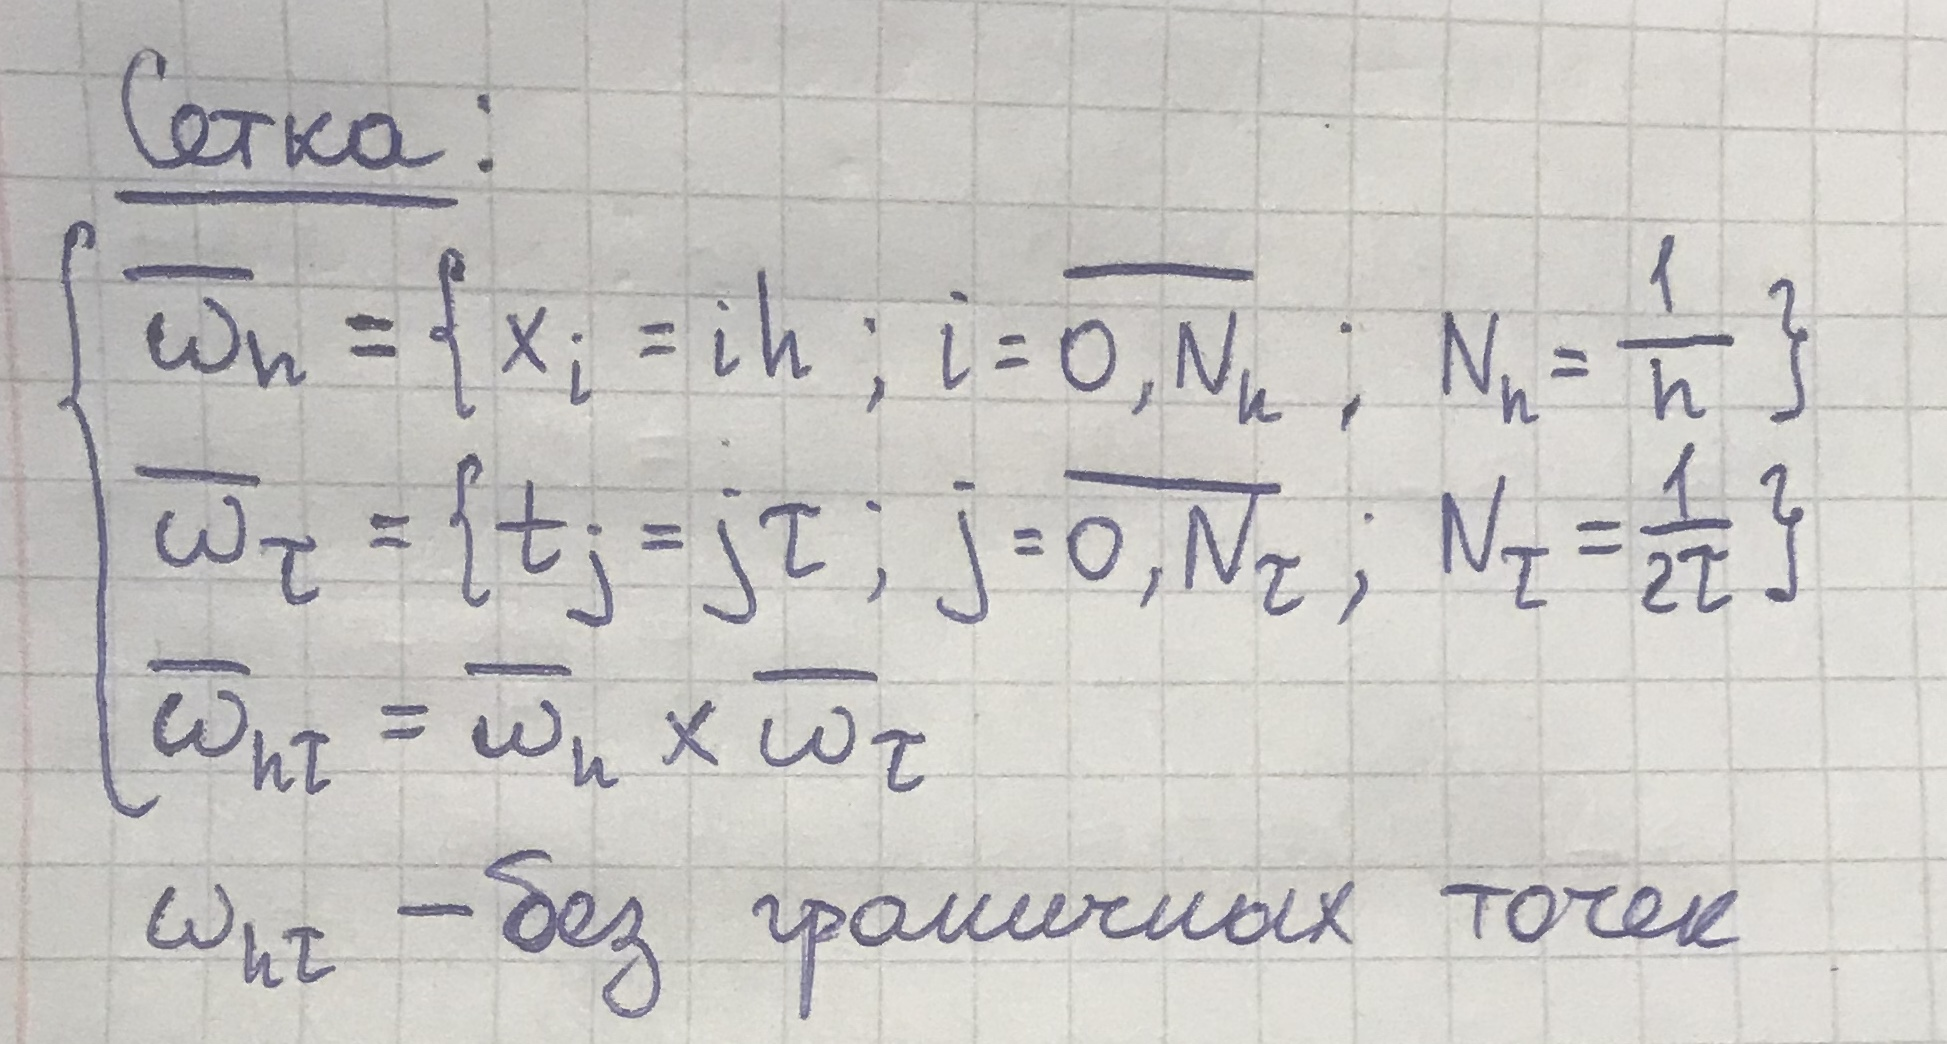
\includegraphics[scale=0.1]{img00.JPG}

\item%
\underline{Разностные схемы}

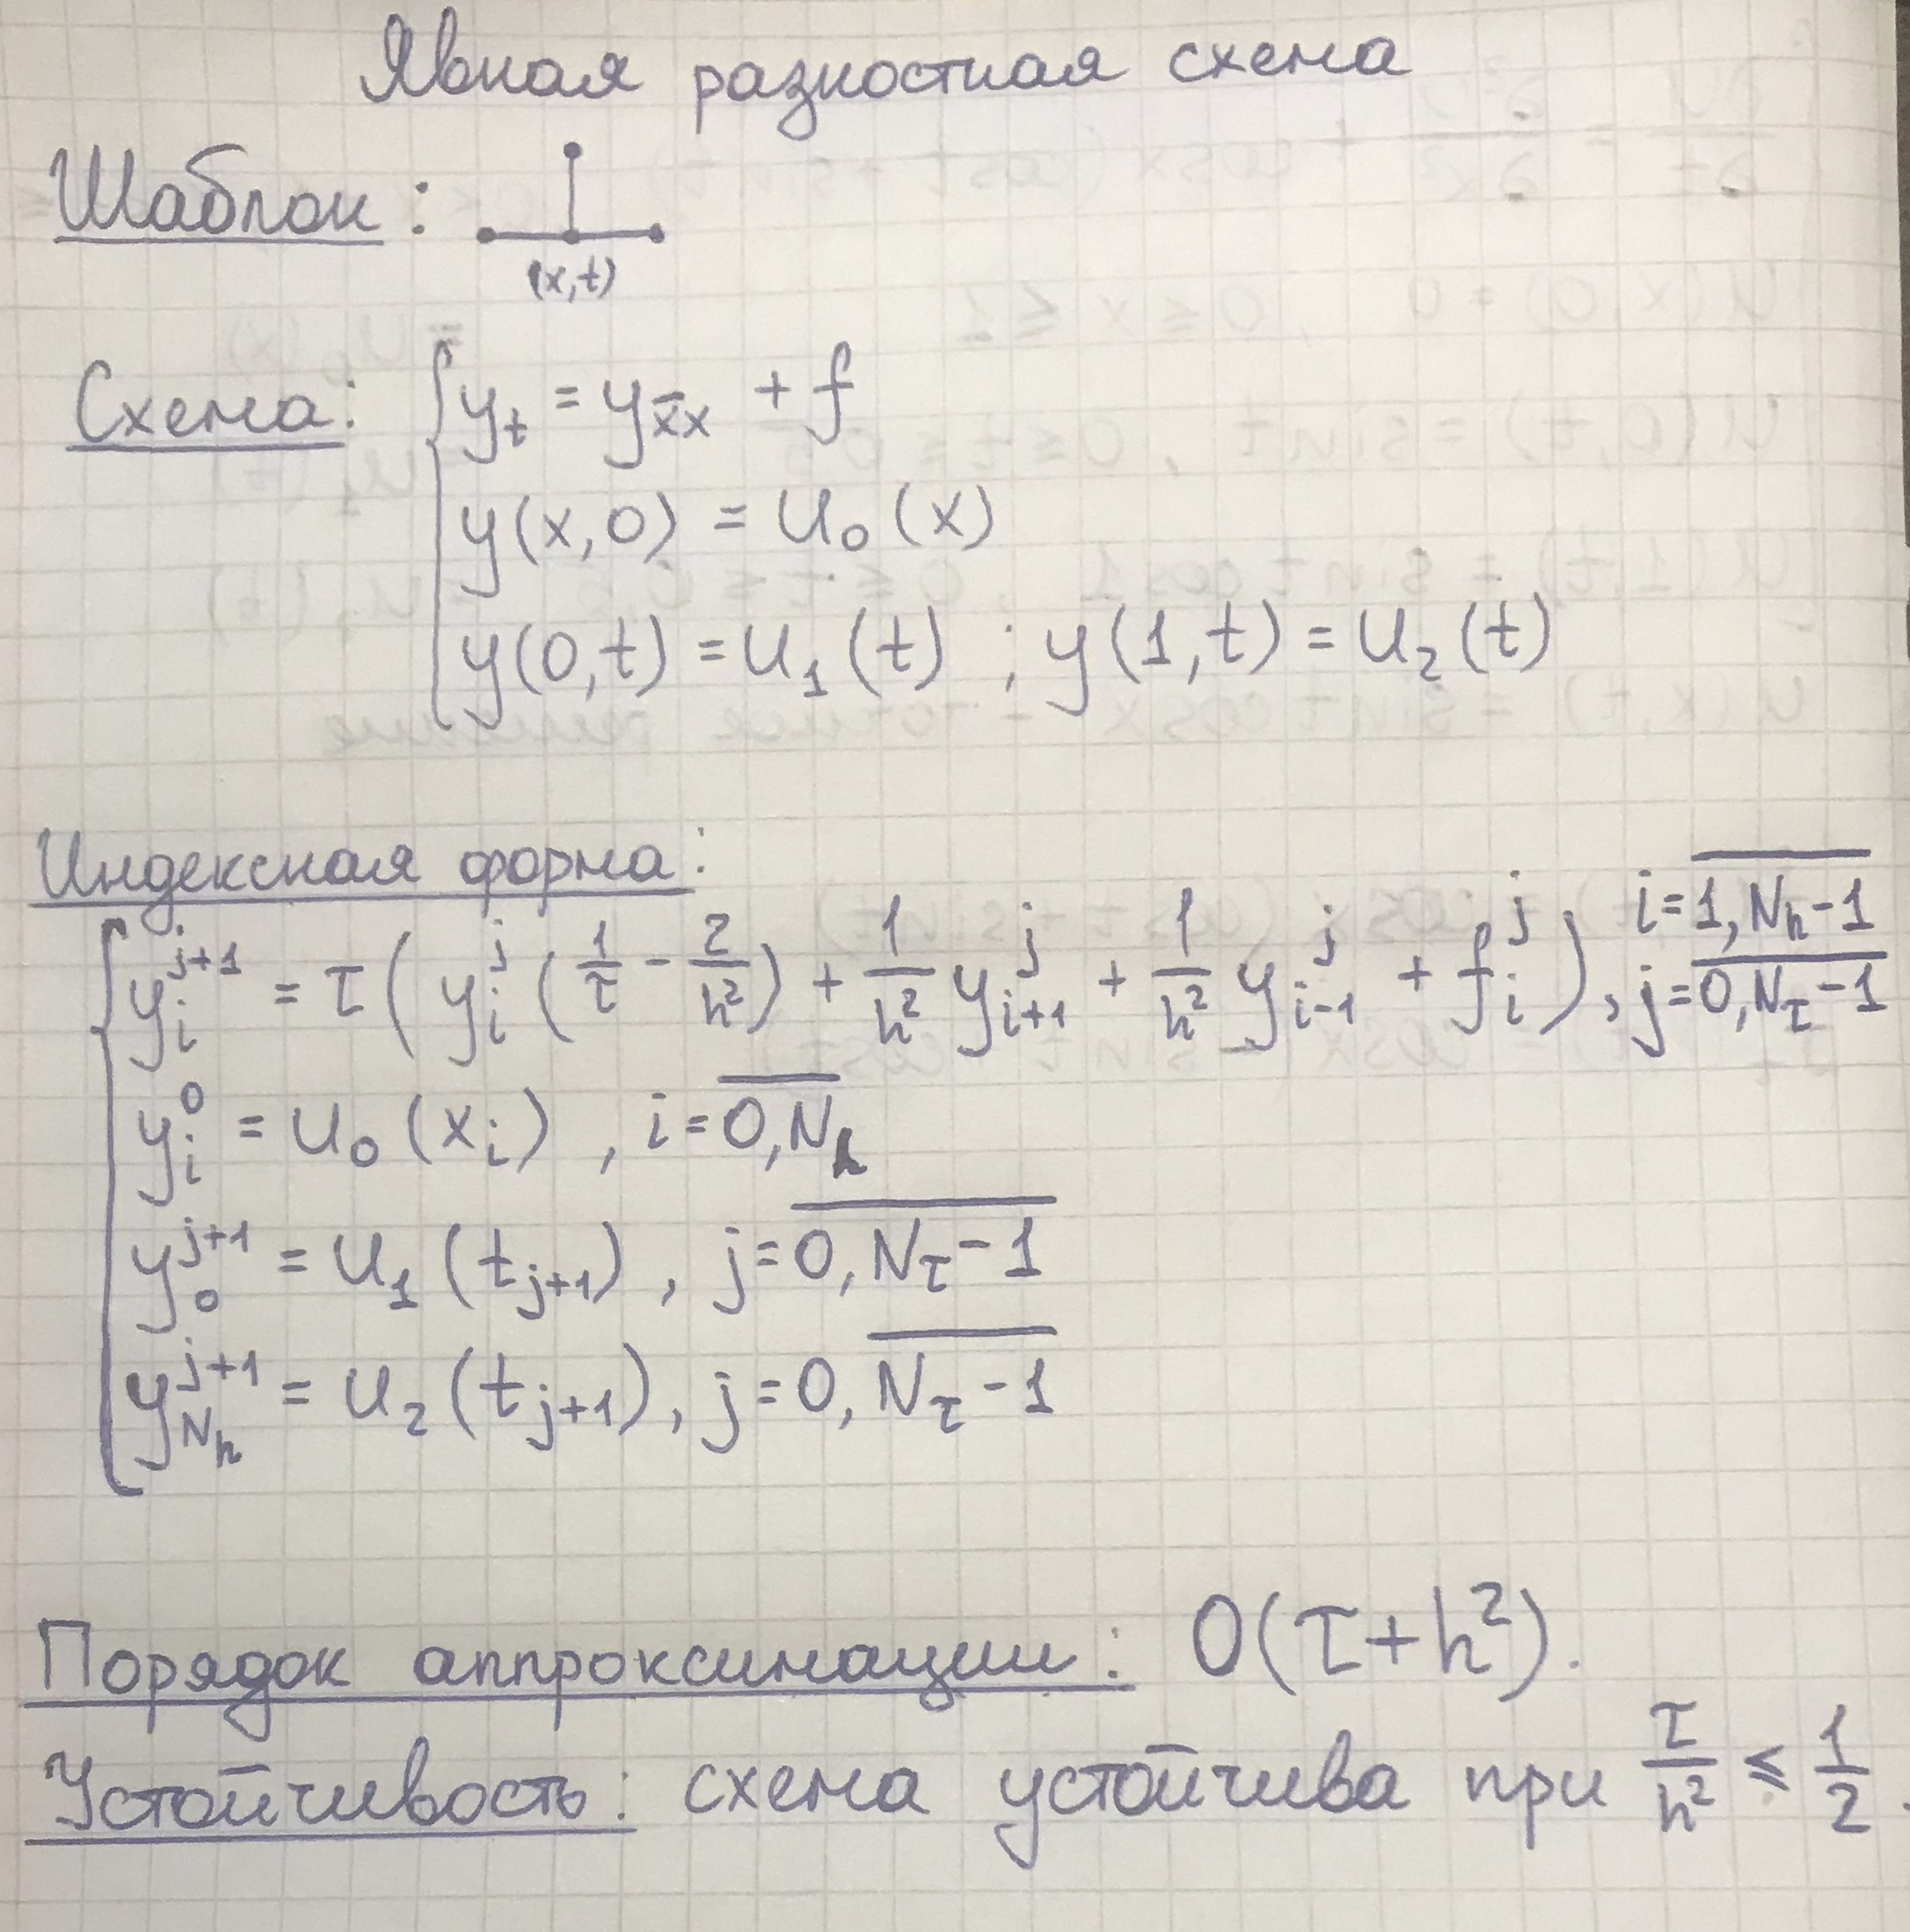
\includegraphics[scale=0.1]{img01.JPG}

В случае $h=\tau=0.1$ явная разностная схема является неустойчивой.

Полученная погрешность: $\Delta = 0.6273$

3D-график численного решения:

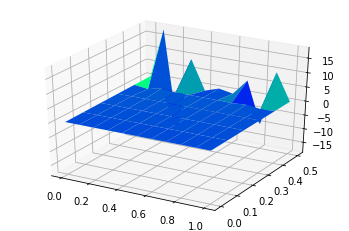
\includegraphics[scale=0.7]{output_12_0.png}

Рассмотрим также сечение в момент времени $t=0.4$ (зеленым - точное решение, красным - численное):

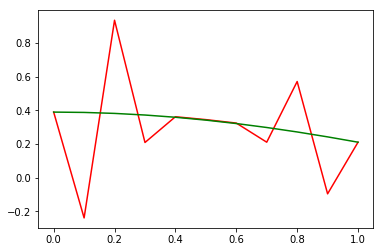
\includegraphics[scale=0.7]{output_13_1.png}

По графикам хорошо видно неустойчивое поведение схемы при заданных параметрах. 

Теперь рассмотрим ту же схему с $h=0.1, \tau=\frac{h^2}{2}=0.005$.

Полученная погрешность: $\Delta = 0.00014$

3D-график численного решения:

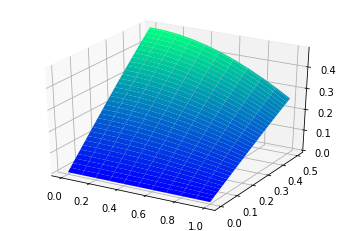
\includegraphics[scale=0.7]{output_16_0.png}

При таких параметрах схема устойчива и решение представляет собой гладкую поверхность.

\clearpage

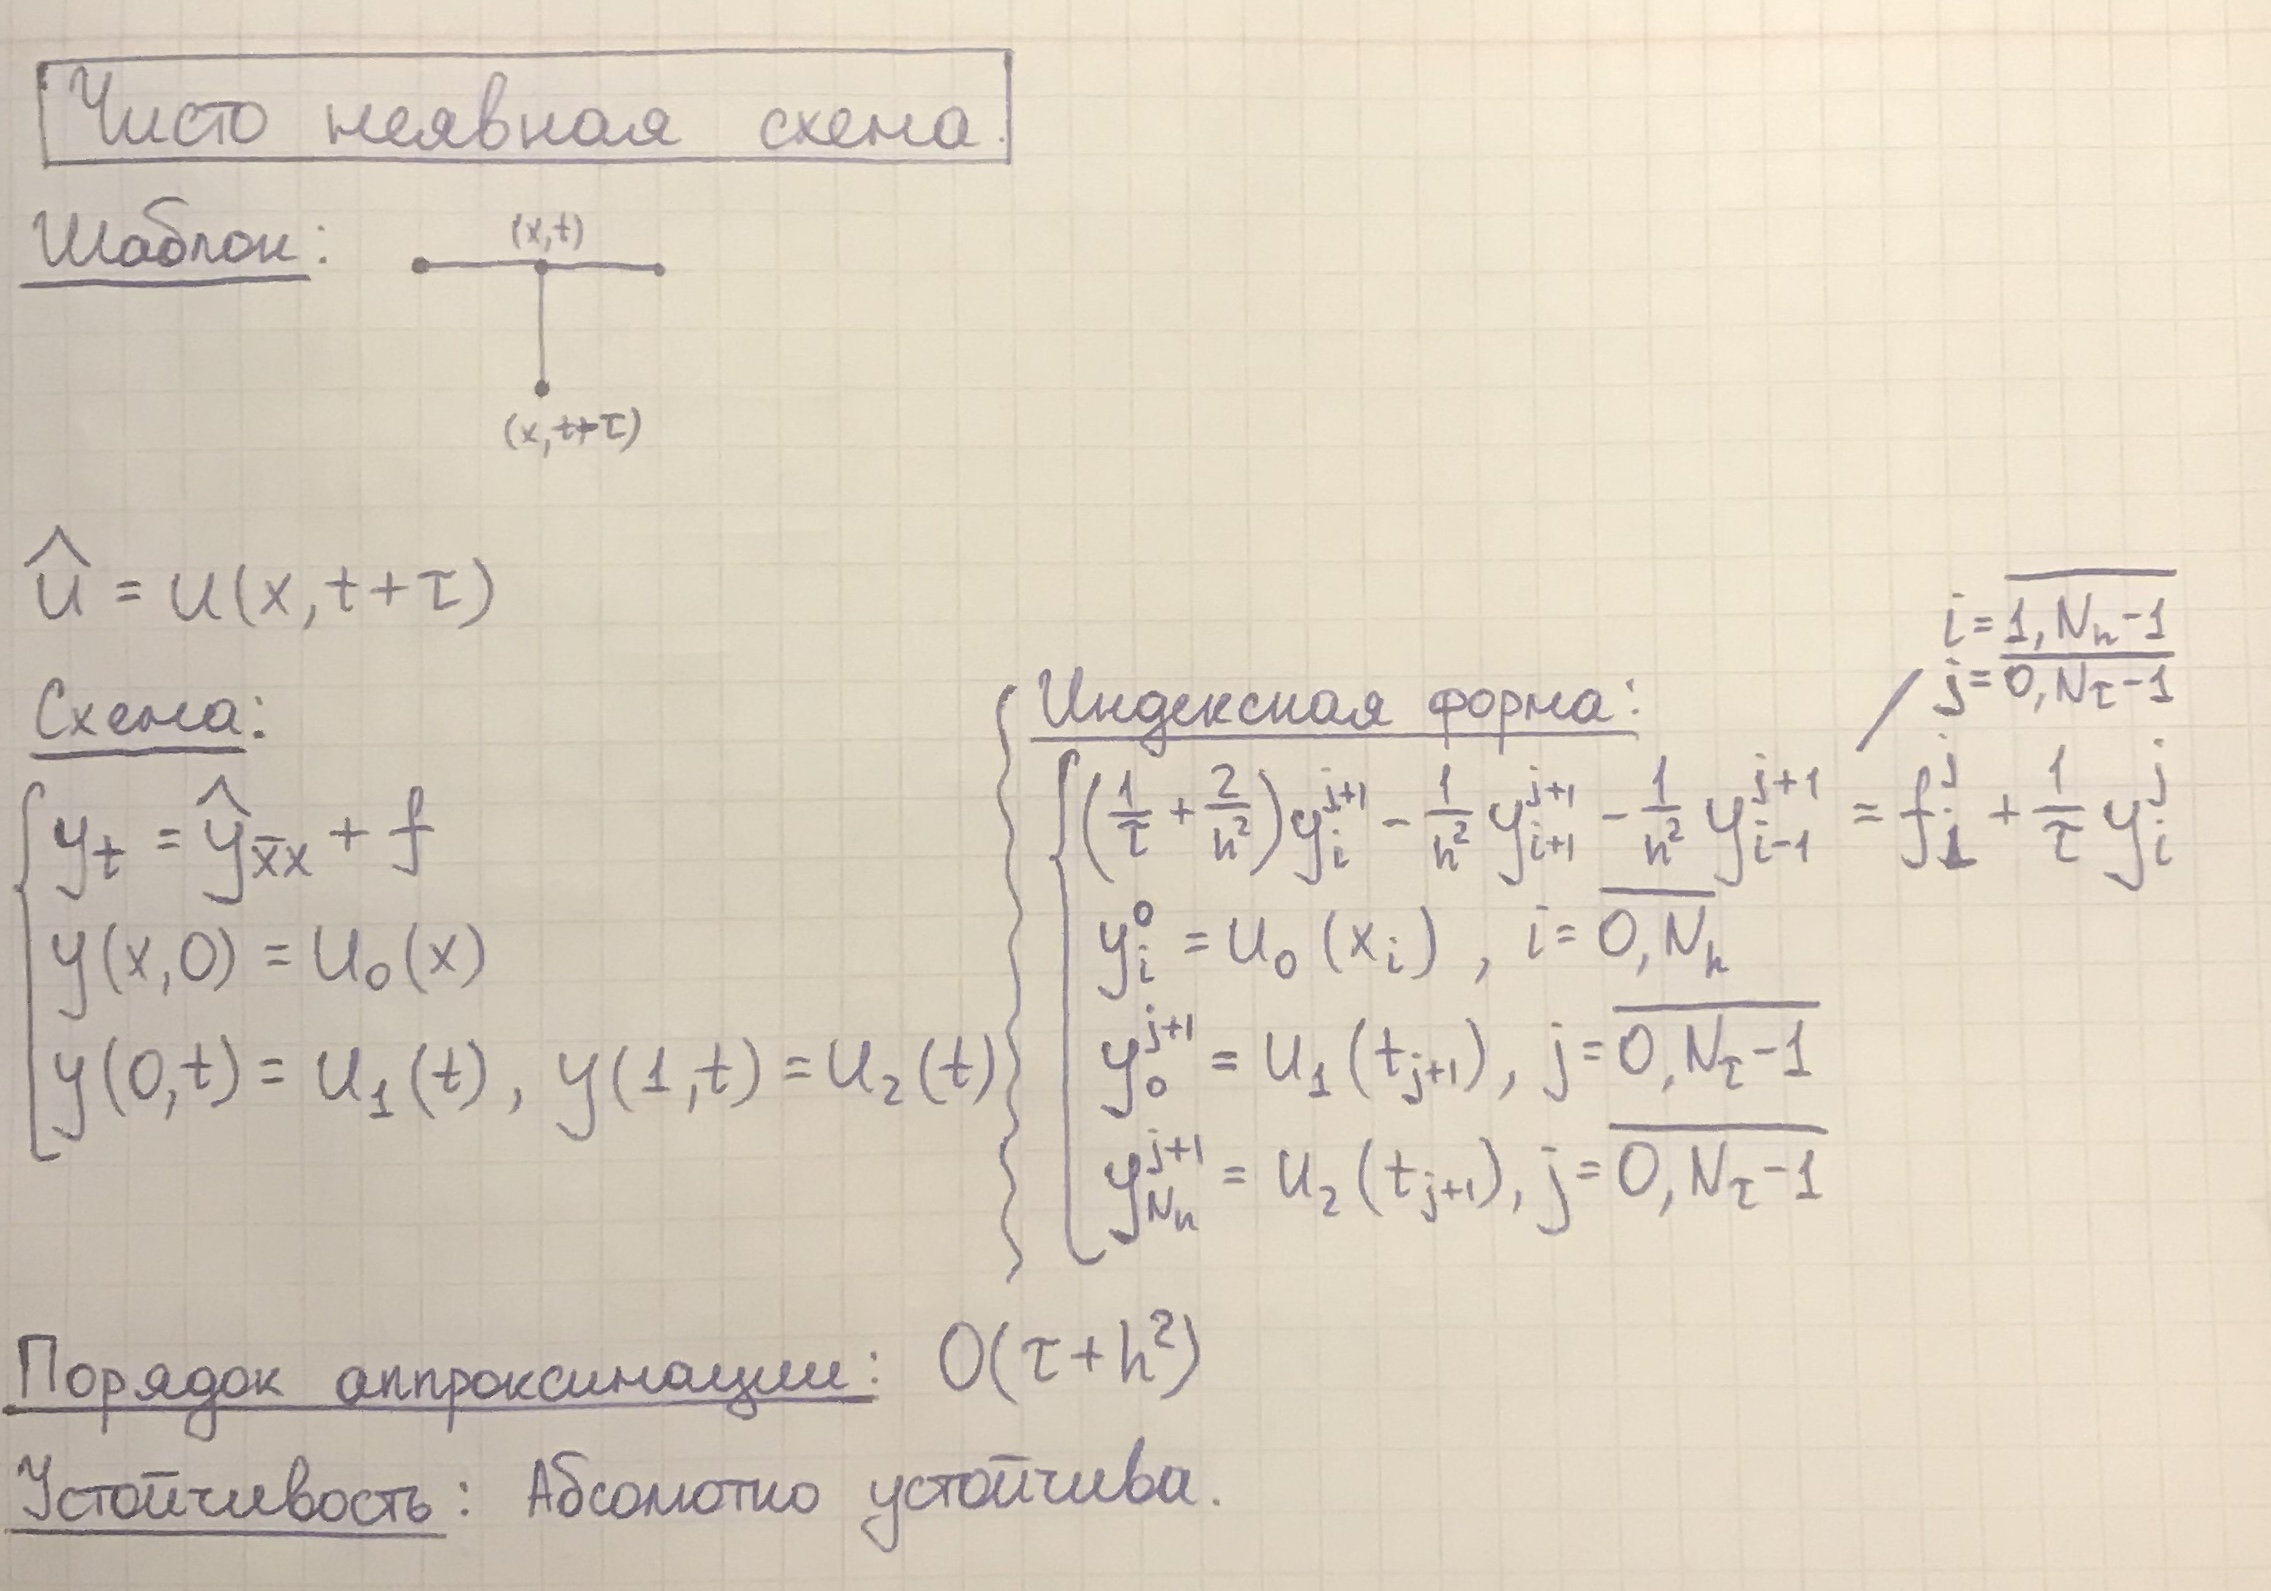
\includegraphics[scale=0.16]{img02.JPG}

Полученная погрешность: $\Delta = 0.00831$

Cечение в момент времени $t=0.4$ (зеленым - точное решение, красным - численное) демонстрирует устойчивое поведение схемы:

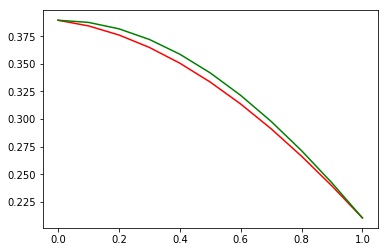
\includegraphics[scale=0.7]{output_20_1.png}

3D-график численного решения:

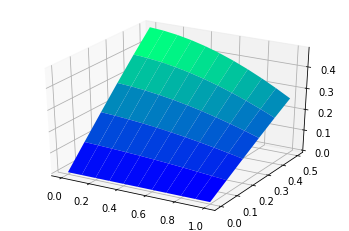
\includegraphics[scale=0.7]{output_19_0.png}

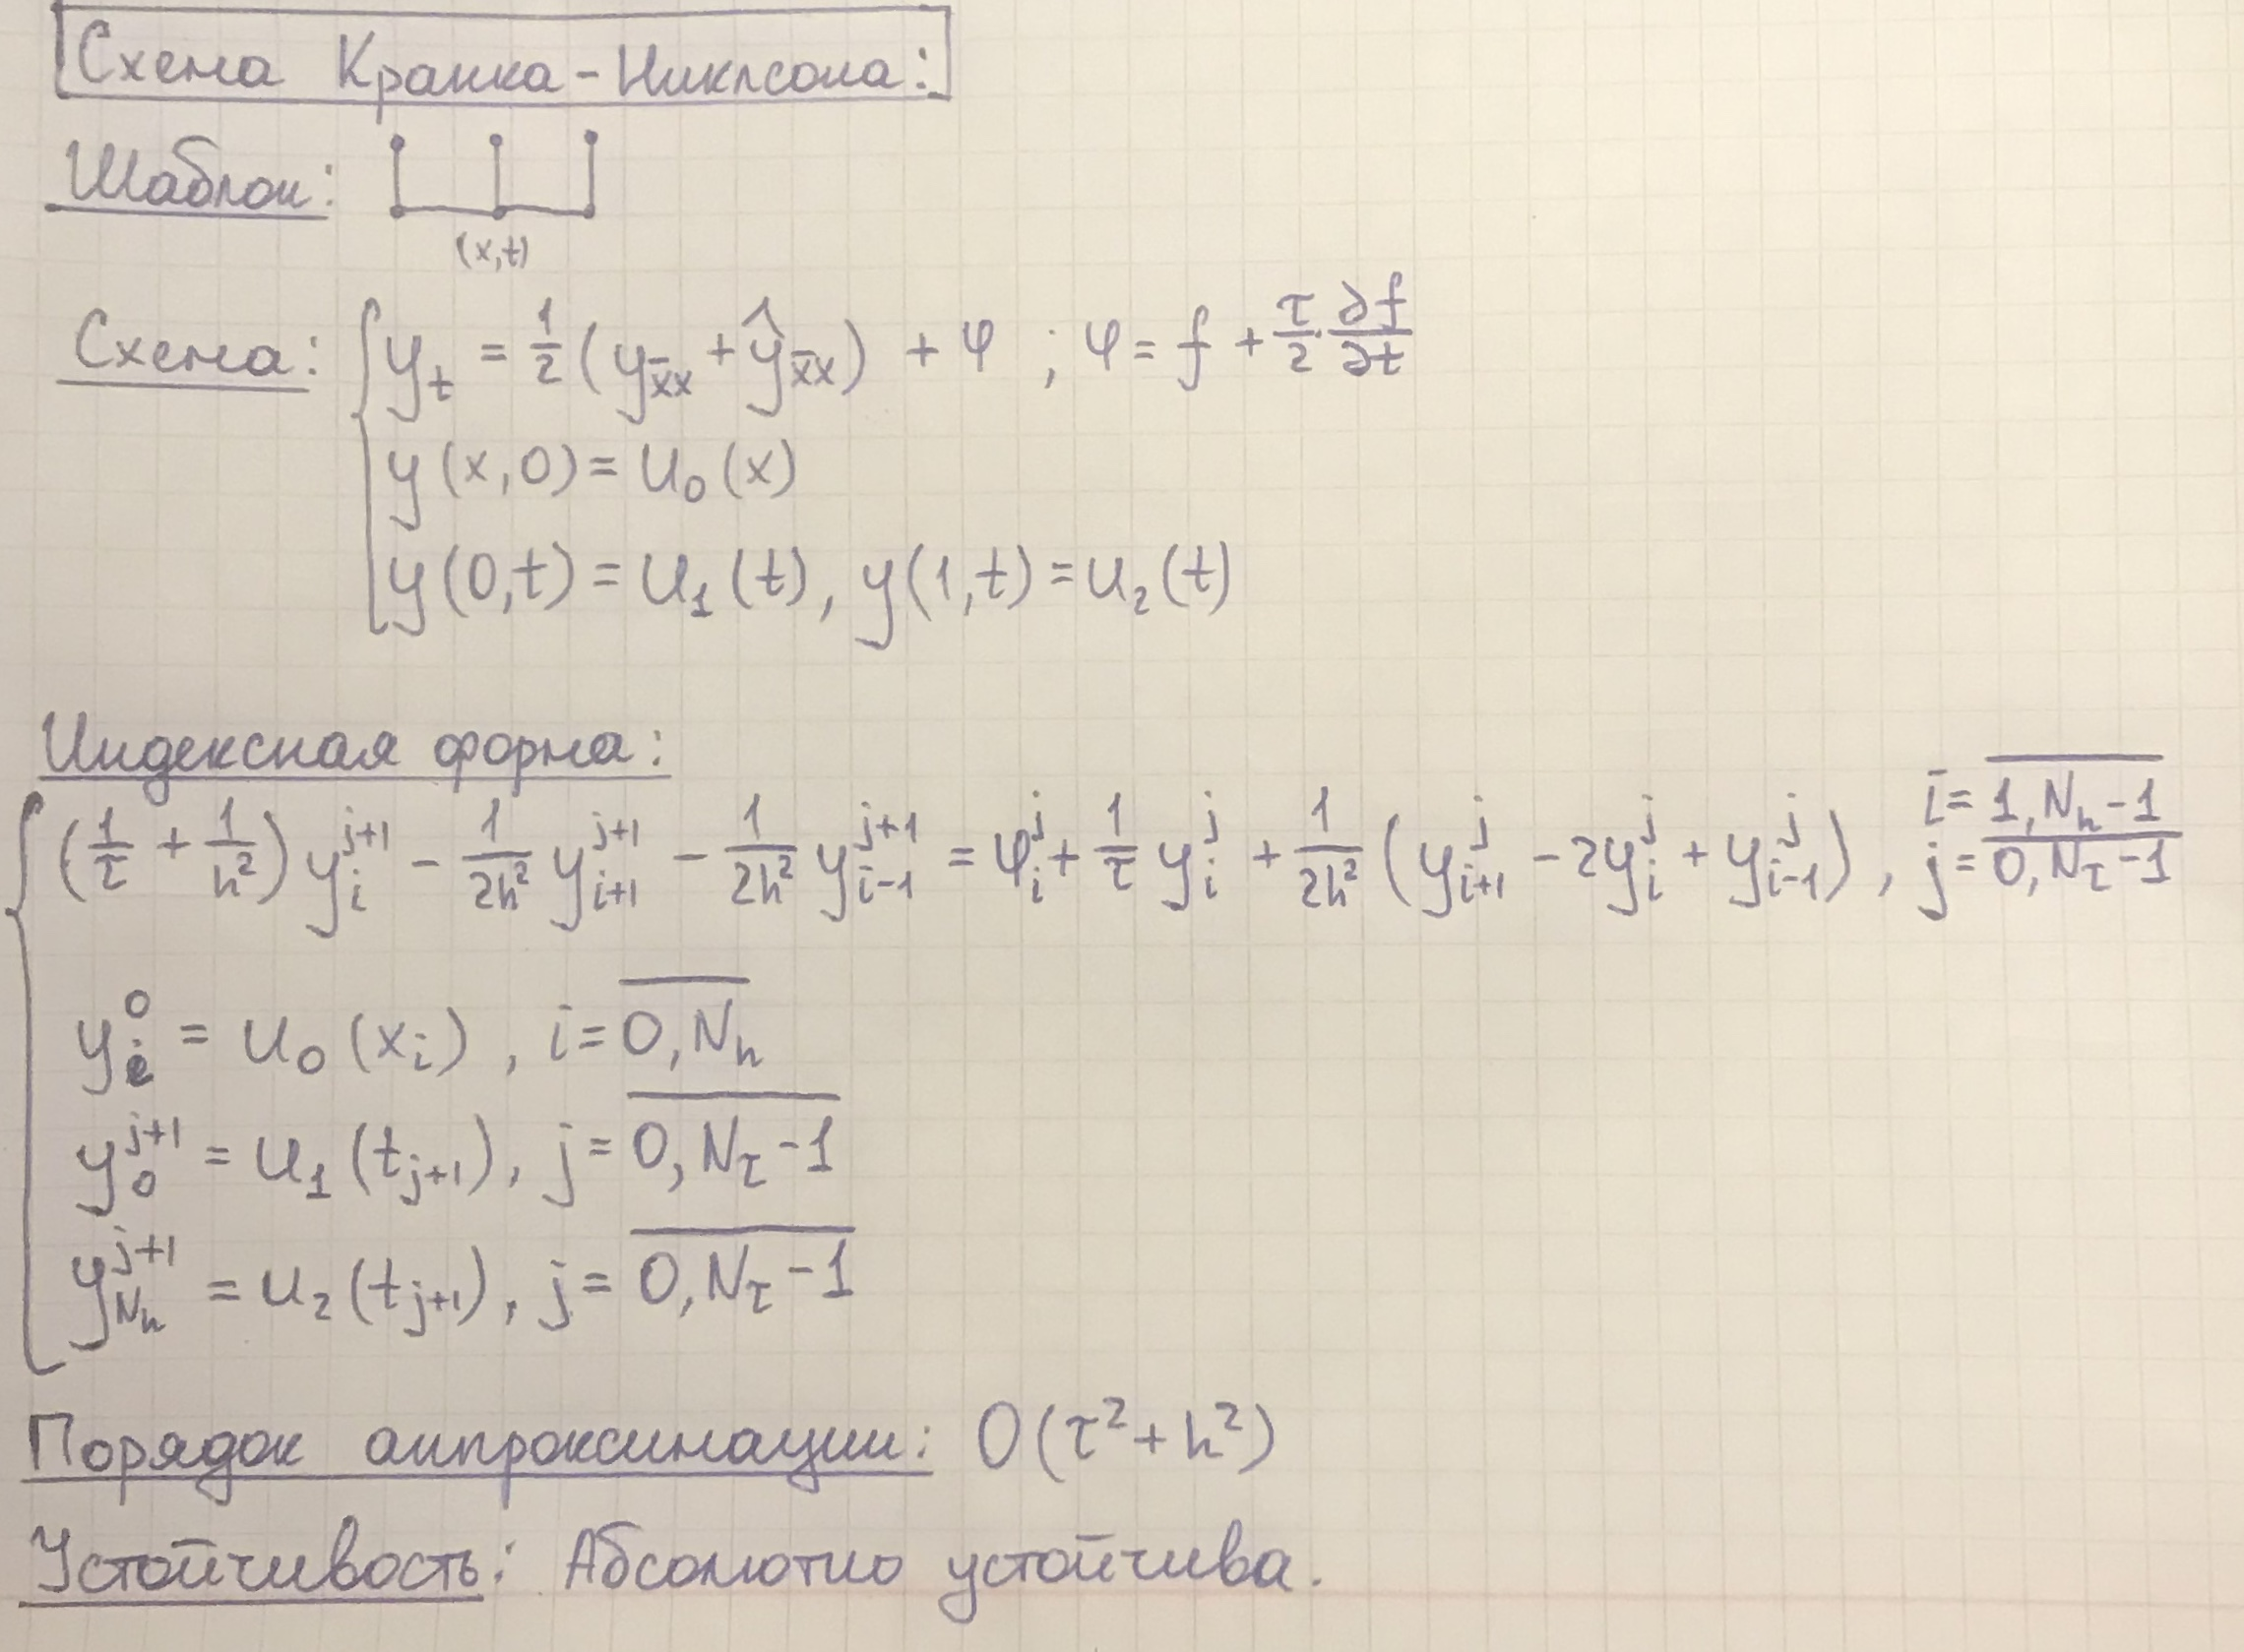
\includegraphics[scale=0.16]{img03.JPG}

Полученная погрешность: $\Delta = 0.00027$

\item%
\underline{Листинг программы}

\begin{scriptsize}
\begin{verbatim}
import numpy as np
import pandas as pd
from matplotlib import pyplot as plt

def f(x, t):
    return np.cos(x) * (np.cos(t) + np.sin(t))

def u0(x):
    return 0

def u1(t):
    return np.sin(t)

def u2(t):
    return np.sin(t) * np.cos(1)

def u(x, t):
    return np.sin(t) * np.cos(x)

def phi(x, t, tau):
    return f(x, t) + (tau/2)*(np.cos(x) * (np.cos(t) - np.sin(t)))

def solve_tridiagonal_1(x, ypast, h, tau, t):
    N = x.shape[0] - 1
    a = np.zeros(N+1)
    c = np.zeros(N+1)
    b = np.zeros(N+1)
    F = np.zeros(N+1)
    
    b[0] = 0
    c[0] = 1
    F[0] = u1(t+tau)
    
    c[N] = 1
    a[N] = 0
    F[N] = u2(t+tau)
    
    for j in range(1,N):
        a[j] = 1/(h*h)
        c[j] = 2/(h*h) + 1/tau
        b[j] = 1/(h*h)
        F[j] = f(x[j], t) + (1/tau)*ypast[j]
        
    alpha = np.zeros(N+1)
    beta = np.zeros(N+2)
    
    alpha[1] = b[0]/c[0]
    beta[1] = F[0]/c[0]
    
    for i in range(1, N):
        alpha[i+1] = b[i]/(c[i] - a[i]*alpha[i])
        beta[i+1] = (F[i] + a[i]*beta[i])/(c[i] - a[i]*alpha[i])
        
    beta[N+1] = (F[N] + a[N]*beta[N])/(c[N] - a[N]*alpha[N])
        
    y = np.zeros(N+1)
    
    y[N] = beta[N+1]
    for i in reversed(range(0, N)):
        y[i] = alpha[i+1]*y[i+1] + beta[i+1]
        
    return y

def solve_tridiagonal_2(x, ypast, h, tau, t):
    N = x.shape[0] - 1
    a = np.zeros(N+1)
    c = np.zeros(N+1)
    b = np.zeros(N+1)
    F = np.zeros(N+1)
    
    b[0] = 0
    c[0] = 1
    F[0] = u1(t+tau)
    
    c[N] = 1
    a[N] = 0
    F[N] = u2(t+tau)
    
    for j in range(1,N):
        a[j] = 1/(2*h*h)
        c[j] = 1/(h*h) + 1/tau
        b[j] = 1/(2*h*h)
        F[j] = phi(x[j], t, tau) + (1/tau)*ypast[j] + 1/(2*h*h)*(ypast[j+1] - 2*ypast[j] + ypast[j-1])
        
    alpha = np.zeros(N+1)
    beta = np.zeros(N+2)
    
    alpha[1] = b[0]/c[0]
    beta[1] = F[0]/c[0]
    
    for i in range(1, N):
        alpha[i+1] = b[i]/(c[i] - a[i]*alpha[i])
        beta[i+1] = (F[i] + a[i]*beta[i])/(c[i] - a[i]*alpha[i])
        
    beta[N+1] = (F[N] + a[N]*beta[N])/(c[N] - a[N]*alpha[N])
        
    y = np.zeros(N+1)
    
    y[N] = beta[N+1]
    for i in reversed(range(0, N)):
        y[i] = alpha[i+1]*y[i+1] + beta[i+1]
        
    return y

from mpl_toolkits.mplot3d import Axes3D
from matplotlib import cm

def plot_answer(X, Y, Z):
    fig = plt.figure()
    ax = fig.add_subplot(111, projection='3d')

    X, Y = np.meshgrid(X, Y)

    surf = ax.plot_surface(X, Y, Z, cmap=cm.winter,
                       linewidth=3, antialiased=True)

    plt.show()

def make_table(h, tau):
    tn, hn = int(0.5/tau) + 1, int(1/h) + 1
    return np.zeros((tn, hn))

def make_grid(h, tau):
    xgrid = np.linspace(0, 1, int(1/h)+1, True)
    tgrid = np.linspace(0, 0.5, int(0.5/tau)+1, True)
    return xgrid, tgrid

xgrid, tgrid = make_grid(0.1, 0.1)
xgrid2, tgrid2 = make_grid(0.1, 0.005)

y1 = make_table(0.1, 0.1)
y2 = make_table(0.1, 0.005)
y3 = make_table(0.1, 0.1)
y4 = make_table(0.1, 0.1)

def get_error(y, xgrid, tgrid):
    error = 0.0
    for i in range(0, len(tgrid) - 1):
        for j in range(0, len(xgrid) - 1):
            if (error < np.abs(y[i][j] - u(xgrid[j], tgrid[i]))):
                error = np.abs(y[i][j] - u(xgrid[j], tgrid[i]))
    return error

tau = 0.1
h = 0.1
for j in range(0, len(xgrid)):
    y1[0][j] = u0(xgrid[j])  
for i in range(0, len(tgrid)):
    y1[i][0] = u1(tgrid[i])
    y1[i][len(xgrid) - 1] = u2(tgrid[i])   
for i in range(0, len(tgrid) - 1):
    for j in range(1, len(xgrid) - 1):
        y1[i+1][j] = tau * (y1[i][j]*(1/tau - 2/(h*h)) + y1[i][j+1]/(h*h) + y1[i][j-1]/(h*h) + f(xgrid[j], tgrid[i]))
print(get_error(y1, xgrid, tgrid))

plot_answer(xgrid, tgrid, y1[:])
plt.plot(xgrid, y1[4], 'r', xgrid, u(xgrid, tgrid[4]), 'g')

tau = 0.005
h = 0.1
for j in range(0, len(xgrid2)):
    y2[0][j] = u0(xgrid2[j])
for i in range(0, len(tgrid2)):
    y2[i][0] = u1(tgrid2[i])
    y2[i][len(xgrid2) - 1] = u2(tgrid2[i])  
for i in range(0, len(tgrid2) - 1):
    for j in range(1, len(xgrid2) - 1):
        y2[i+1][j] = tau * (y2[i][j]*(1/tau - 2/(h*h)) + y2[i][j+1]/(h*h) + y2[i][j-1]/(h*h) + f(xgrid2[j], tgrid2[i]))
print(get_error(y2, xgrid2, tgrid2))

plot_answer(xgrid2, tgrid2, y2[:])

tau = 0.1
h = 0.1
for j in range(0, len(xgrid)):
    y3[0][j] = u0(xgrid[j])
for i in range(0, len(tgrid) - 1):
    y3[i+1] = solve_tridiagonal_1(xgrid, y3[i], h, tau, tgrid[i])
print(get_error(y3, xgrid, tgrid))

plot_answer(xgrid, tgrid, y3[:])
plt.plot(xgrid, y3[4], 'r', xgrid, u(xgrid, tgrid[4]), 'g')

tau = 0.1
h = 0.1
for j in range(0, len(xgrid)):
    y4[0][j] = u0(xgrid[j])   
for i in range(0, len(tgrid) - 1):
    y4[i+1] = solve_tridiagonal_2(xgrid, y4[i], h, tau, tgrid[i])
print(get_error(y4, xgrid, tgrid))
\end{verbatim}
\end{scriptsize}

\end{enumerate}%
\end{document}